% % % % % % % % % % % % % % % % % % % % % % % % % % % % % % % % % % % % %
% Chapter: Experiment 1
% % % % % % % % % % % % % % % % % % % % % % % % % % % % % % % % % % % % %
\chapter{Experiment 1: Using random input}
\label{chp:experiment1}
% Explain something like method? 
% Or maybe a sort of introduction to describe the property-based testing we do in the first case

% % % % % % % % % % % % % % % % % % % % % % % % % % % % % % % % % % % % %
% Section: Initial case
%\section{Initial case}
%\label{sec:initial_case}
\pinfo{Props to test cases, implication returns True}
The properties that we defined in \autoref{cpt:4_properties} are translated into test cases as described in \autoref{cpt:3_testmechanics}. For the properties that use implication ($\implies$) an if-else statement is created. The else-statement will return \textit{True} just like the definition of implication\todo{Add source}.\\
\\
\pinfo{Like QuickCheck, recall cycle shortly}
In the first experiment each property will be tested 100 times with random input values. This is a similar approach as what QuickCheck does with checking properties. The methods to generate the random value pairs are added to the template of a test file. A full test run consists of multiple steps, as described in \autoref{sct:ch3_full_cycle}. In short these steps are: building the specifications, generating the system, generating the test suit and as last run the generated test suit.

% % % % % % % % % % % % % % % % % % % % % % % % % % % % % % % % % % % % %
% Section: First run
\section{First run}
\pinfo{Termination, compile error due to library}
The first run resulted into a termination of the run due to a compile error in the generated system. Although we made the assumption that the generated system should be compilable, this error came from a property definition that was expected to fulfill, namely \textit{AssociativeMultiplicationInteger1}. Which is why we can consider this as an error. The error describes that an overloaded method cannot be applied to the \textit{Money} type, as shown in \autoref{lst:ch5_firstrun_termination_log}.
\\
% Listing
\begin{sourcecode}[h!]
\begin{lstlisting}[language=Log]
[error] MoneySpec.scala:316: overloaded method value * with alternatives:
[error]   (x: Double)Double <and>
[error]   (x: Float)Float <and>
[error]   (x: Long)Long <and>
[error]   (x: Int)Int <and>
[error]   (x: Char)Int <and>
[error]   (x: Short)Int <and>
[error]   (x: Byte)Int
[error]  cannot be applied to (squants.market.Money)
[error]           Initialised(Data(result = Some(((((x * y)) * z) == (x * ((y * z)))))))
[error]                                                                 ^
[error] MoneySpec.scala:441: overloaded method value * with alternatives:
[error]   (x: Double)Double <and>
[error]   (x: Float)Float <and>
[error]   (x: Long)Long <and>
[error]   (x: Int)Int <and>
[error]   (x: Char)Int <and>
[error]   (x: Short)Int <and>
[error]   (x: Byte)Int
[error]  cannot be applied to (squants.market.Money)
[error]             checkPostCondition((nextData.get.result.get == (((((x * y)) * z) == (x * ((y * z)))))), "new this.result == ( (x*y)*z == x*(y*z) )")
[error]                                                                                    ^
[error] two errors found
[error] (compile:compileIncremental) Compilation failed
[error] Total time: 79 s, completed 4-aug-2017 13:03:45
> Done testing
> ** Some tests failed! **
\end{lstlisting}
\caption{Log output first test run resulting in a termination.}
\label{lst:ch5_firstrun_termination_log}
\end{sourcecode}
\todo{Up arrow is incorrectly aligned in the listing due to layout}
% End listing
\\
\pinfo{Investigation, found property and var types}
The error log does not clearly indicate what is exactly going wrong, it also does not describe what the types of the variables were. Investigating the generated system reveals that both errors were happening when dealing with the \textit{AssociativeMultiplicationInteger1} property. This means that the variables x, y and z are of type \textit{Integer}, \textit{Integer}, \textit{Money} respectively, as described in \autoref{ssct:ch2_money_associativity}.\\
\\
\pinfo{Created issue in Squants, now proceed}
For the \textit{Money} type, an open source library is used called Squants\footnote{https://github.com/typelevel/squants}. The missing method was actually an issue within this library. This means that in order to proceed further, a fix in the library would be required. For this we created an issue on Github describing the problem\footnote{https://github.com/typelevel/squants/issues/281}. In order to proceed with our test suit, we temporary disable this property till a fix has been made in the Squants library.

% % % % % % % % % % % % % % % % % % % % % % % % % % % % % % % % % % % % %
% Section: Second run
\section{Second run}
\pinfo{Failing tests, describing each}
After disabling the \textit{AssociativeMultiplicationInteger1} property, the test suit was able to run completely. The result was 7 failing tests. For each test the input values are logged such that the error can be reproduced. For each test we describe the investigation of what went wrong. After that, the results of our test suit can be evaluated.\\
\\
The first four tests reveal precision problems when using the \textit{Money} type in calculations. The latter three tests were initially also failing because of these precision problems. However, these tests were also failing after the precision errors were fixed. For the latter 3 tests another version of the generated system was used, which contains the fixes for the precision problems. This is done so that we were able to reveal the other errors that these properties reveal.

\todo{Add red and bold in tables}
% % %
% Explaining failing cases.
% % %
% % %
% DistributivePercentage1
\subsection{DistributivePercentage1}
\label{ssct:ch5_distributivePercentage1}
This property uses a \textit{Percentage} value and two \textit{Money} values for it's tests. The values are named x, y and z respectively. To check this failing test, we check the results of the intermediate calculations in the formula that is being used. In \autoref{ch4_init_check_DistributivePercentage1} values are shown for which the test case fails, among with the intermediate calculations. The intermediate calculations seem to work as expected, as the results are the same when we compare the results of the Scala evaluation and the Rascal evaluation. Unfortunately the resulting left hand side of the expression contains a precision error, which is caused when multiplying a \textit{Percentage} (the x variable) with a \textit{Money} type (the result of y+z in this case).
% Table: Values of DistributivePercentage1
\FloatBarrier
\begin{table}[h!]
\centering
\begin{tabular}{|lll|}
\hline
\multicolumn{3}{|c|}{DistributivePercentage1}                          \\ \hline
Variable   -            & Value                   & Type                \\
\multicolumn{1}{|r}{X} & 0.51                    & Percentage          \\
\multicolumn{1}{|r}{Y} & -311254801.77 EUR       & Money               \\
\multicolumn{1}{|r}{Z} & -707194075.77 EUR       & Money               \\ \hline
Formula                & Scala result            & Expected result     \\
x*(y+z) == (y*x)+(z*x) & false                   & true                \\
x*(y+z)                & -519408927.54539996 EUR & -519408927.5454 EUR \\
(y*x)+(z*x)            & -519408927.5454 EUR     & -519408927.5454 EUR \\
                       &                         &                     \\
y+z                    & -1018448877.54 EUR      & -1018448877.54 EUR  \\
y*x                    & -158739948.9027 EUR     & -158739948.9027 EUR \\
z*x                    & -360668978.6427 EUR     & -360668978.6427 EUR \\ \hline
\end{tabular}
\caption{DistributivePercentage1: Precision error when multiplying a \textit{Percentage} with \textit{Money}}
\label{ch4_init_check_DistributivePercentage1}
\end{table}
\FloatBarrier

% % %
% DistributivePercentage2
\subsection{DistributivePercentage2}
This test case looks similar than the \textit{DistributivePercentage1} (\autoref{ssct:ch5_distributivePercentage1}). It uses the same type of variables, but the expression is slightly different. In \autoref{ch4_init_check_DistributivePercentage2} the result and the intermediate calculations of a failing case are shown. What can be seen here is that the precision error occurs when the Money type is multiplied by the Percentage type. While in \autoref{ssct:ch5_distributivePercentage1} it was the other way around.
\\
\begin{table}[h!]
\centering
\begin{tabular}{|lll|}
\hline
\multicolumn{3}{|c|}{DistributivePercentage2}                           \\ \hline
Variable               & Value                   & Type                 \\
\multicolumn{1}{|r}{X} & 0.93                    & Percentage           \\
\multicolumn{1}{|r}{Y} & 2089630160.75 EUR       & Money                \\
\multicolumn{1}{|r}{Z} & -1316628389.49 EUR      & Money                \\ \hline
Formula                & Scala result            & Expected result      \\
(y+z)*x == (y*x)+(z*x) & false                   & true                 \\
(y+z)*x                & 718891647.2718 EUR      & 718891647.2718 EUR   \\
(y*x)+(z*x)            & 718891647.2718001 EUR   & 718891647.2718 EUR   \\
                       &                         &                      \\
y+z                    & 773001771.26 EUR        & 773001771.26 EUR     \\
y*x                    & 1943356049.4975002 EUR  & 1943356049.4975 EUR  \\
z*x                    & -1224464402.2257001 EUR & -1224464402.2257 EUR \\ \hline
\end{tabular}
\caption{DistributivePercentage1: Precision error when multiplying a \textit{Money} with \textit{Percentage}}
\label{ch4_init_check_DistributivePercentage2}
\end{table}
\\

% % %
% DistributiveInt2
\subsection{DistributiveInt2}
\label{ssct:ch5_distributiveInt2}
This case uses \textit{Integer} in conjunction with the \textit{Money} type. Earlier cases showed that there was a precision error when using the \textit{Percentage} and \textit{Money} types. Since the \textit{Percentage} type is translated to a \textit{Double} in the generated system, it can be expected that there would be precision problems occuring. As this is a known issue with types that use floating-point arithmetic \cite{goldberg1991every}. This case reveals that a precision error also occurs when multiplying \textit{Money} with an \textit{Integer}. In the intermediate calculations when investigating a failing test with it's values are shown in \autoref{ch4_init_check_DistributiveInt2}. The last two rows, colored in red, show that a precision error occurs when \textit{Money} is multiplied by an \textit{Integer}.
\\
\begin{table}[h!]
\centering
\begin{tabular}{lll}
\hline
\multicolumn{3}{|c|}{DistributiveInt2}                                                                                \\ \hline
\multicolumn{1}{|l}{Variable}           & Value                   & \multicolumn{1}{l|}{Type}                       \\
\multicolumn{1}{|r}{X}                  & -883022216              & \multicolumn{1}{l|}{Integer}                    \\
\multicolumn{1}{|r}{Y}                  & -298435082.93 EUR       & \multicolumn{1}{l|}{Money}                      \\
\multicolumn{1}{|r}{Z}                  & 715725888.96 EUR        & \multicolumn{1}{l|}{Money}                      \\ \hline
\multicolumn{1}{|l}{Formula}            & Scala result            & \multicolumn{1}{l|}{Expected result}            \\
\multicolumn{1}{|l}{(x*y)*z == x*(y*z)} & false                   & \multicolumn{1}{l|}{true}                       \\
\multicolumn{1}{|l}{(x*y)*z}            & -368477052257036740 EUR & \multicolumn{1}{l|}{-368477052257036762.48 EUR} \\
\multicolumn{1}{|l}{x*(y*z)}            & -368477052257036796 EUR & \multicolumn{1}{l|}{-368477052257036762.48 EUR} \\
\multicolumn{1}{|l}{}                   &                         & \multicolumn{1}{l|}{}                           \\
\multicolumn{1}{|l}{y+z}                & 417290806.03 EUR        & \multicolumn{1}{l|}{417290806.03 EUR}           \\
\multicolumn{1}{|l}{y*x}                & 263524808260992384 EUR  & \multicolumn{1}{l|}{263524808260992372.88 EUR}  \\
\multicolumn{1}{|l}{z*x}                & -632001860518029180 EUR & \multicolumn{1}{l|}{-632001860518029135.36 EUR} \\ \hline
\end{tabular}
\caption{DistributiveInt2: Precision error when multiplying Money with an Integer}
\label{ch4_init_check_DistributiveInt2}
\end{table}
\\

% % %
% AssociativeMultiplicationPercentage2
\subsection{AssociativeMultiplicationPercentage2}
The earlier cases already shown a precision error when using Doubles and Integers in conjunction with \textit{Money}. This case triggers the same problem, but also reveals that the same thing happens when multiplying an \textit{Integer} with \textit{Money}. While in \autoref{ssct:ch5_distributiveInt2} it was the other way around. The intermediate calculations are shown in \autoref{ch4_init_check_AssociativeMultiplicationPercentage2}, the calculation of multiplying an Integer with Money is shown in red. Additionally, this case shows that the small precision error that we've seen earlier can cause a seemingly difference, which is a difference of 130 EUR in this case.
\\
\begin{table}[h!]
\centering
\begin{tabular}{lll}
\hline
\multicolumn{3}{|c|}{AssociativeMultiplicationPercentage2}                                                            \\ \hline
\multicolumn{1}{|l}{Variable}           & Value                   & \multicolumn{1}{l|}{Type}                       \\
\multicolumn{1}{|r}{X}                  & 840296462               & \multicolumn{1}{l|}{Integer}                    \\
\multicolumn{1}{|r}{Y}                  & 1771903729.60 EUR       & \multicolumn{1}{l|}{Money}                      \\
\multicolumn{1}{|r}{Z}                  & 0.53                    & \multicolumn{1}{l|}{Double}                     \\ \hline
\multicolumn{1}{|l}{Formula}            & Scala result            & \multicolumn{1}{l|}{Expected result}            \\
\multicolumn{1}{|l}{(x*y)*z == x*(y*z)} & false                   & \multicolumn{1}{l|}{true}                       \\
\multicolumn{1}{|l}{(x*y)*z}            & 789129950543366910 EUR  & \multicolumn{1}{l|}{789129950543366877.856 EUR} \\
\multicolumn{1}{|l}{x*(y*z)}            & 789129950543366780 EUR  & \multicolumn{1}{l|}{789129950543366877.856 EUR} \\
\multicolumn{1}{|l}{}                   &                         & \multicolumn{1}{l|}{}                           \\
\multicolumn{1}{|l}{x*y}                & 1488924434987484670 EUR & \multicolumn{1}{l|}{1488924434987484675.2 EUR}  \\
\multicolumn{1}{|l}{y*z}                & 939108976.688 EUR       & \multicolumn{1}{l|}{939108976.688 EUR}          \\ \hline
\end{tabular}
\caption{AssociativeMultiplicationPercentage2: Precision error causing bigger differences}
\label{ch4_init_check_AssociativeMultiplicationPercentage2}
\end{table}
\\

% % %
% AssociativeMultiplicationInt2
\subsection{AssociativeMultiplicationInteger2}
% - Integer overflows, causing negative values etc.
For this case three variables are used: x, y and z, which are of type \textit{Money}, \textit{Integer} and \textit{Integer} respectively. In \autoref{ch4_init_check_AssociativeMultiplicationInteger2} the values of a failing test case are shown with the intermediate formula steps. On the left side of the expression we see the expected results, while on the right side there is a big difference. The red colored row shows a huge difference in the resulting values between Scala and the expected value of the intermediate step on this expression. The result value of the operation is smaller than the minimum value of an \textit{Integer}. Causing it to underflow, resulting in an unexpected amount as result. Thus the operation neither checks for underflowing an \textit{Integer} value, nor does it prevent it.\todo{SOURCE-Over/underflow}
% Table: Values of AssociativeMultiplicationInt2
\\
\begin{table}[h!]
\centering
\begin{tabular}{|lll|}
\hline
\multicolumn{3}{|c|}{AssociativeMultiplicationInteger2}                                                \\ \hline
Variable               & Value                               & Type                                \\
\multicolumn{1}{|r}{X} & -1852801029.34 EUR                  & Money                               \\
\multicolumn{1}{|r}{Y} & -1309504561                         & Integer                             \\
\multicolumn{1}{|r}{Z} & 1880170895                          & Integer                             \\ \hline
Formula                & Scala result                        & Expected result                     \\
(x*y)*z == x*(y*z)     & false                               & true                                \\
(x*y)*z                & 4561767263499657218201769467.30 EUR & 4561767263499657218201769467.30 EUR \\
x*(y*z)                & 3877739486117270379.94 EUR          & 4561767263499657218201769467.30 EUR \\
                       &                                     &                                     \\
x*y                    & 2426251398546224819.74 EUR          & 2426251398546224819.74 EUR          \\
y*z                    & -2092906591                         & -2462092362461952095                \\ \hline
\end{tabular}
\caption{AssociativeMultiplicationInteger2: \textit{Integer} underflows when using multiply}
\label{ch4_init_check_AssociativeMultiplicationInteger2}
\end{table}
\\

% % %
% DistributiveInt1
\subsection{DistributiveInt1}
This case also uses three variables: x, y and z. Which are of type \textit{Money}, \textit{Integer} and \textit{Integer} respectively. In \autoref{ch4_init_check_DistributiveInteger1} the different values are shown of the calculation between Scala and the expected result. The red line shows how the addition of two (positive) Integers results in a negative value. The result value would be bigger than the maximum value of an \textit{Integer}, causing it to overflow. Thus the operation also does not check or prevent against overflowing. \todo{SOURCE-Over/underflow}
% Table: Values of DistributiveInt1
\\
\begin{table}[h!]
\centering
\begin{tabular}{|lll|}
\hline
\multicolumn{3}{|c|}{DistributiveInteger1}                                             \\ \hline
Variable               & Value                       & Type                        \\
\multicolumn{1}{|r}{X} & -1790274467.41 EUR          & Money                       \\
\multicolumn{1}{|r}{Y} & 1691684272                  & Integer                     \\
\multicolumn{1}{|r}{Z} & 1449321647                  & Integer                     \\ \hline
Formula                & Scala result                & Expected result             \\
x*(y+z) == (x*y)+(x*z) & false                       & true                        \\
x*(y+z)                & 2065907589620385223.57 EUR  & -5623262698769382599.79 EUR \\
(x*y)+(x*z)            & -5623262698769382599.79 EUR & -5623262698769382599.79 EUR \\
                       &                             &                             \\
y+z                    & -1153961377                 & 3141005919                  \\
x*y                    & -3028579159080673575.52 EUR & -3028579159080673575.52 EUR \\
x*z                    & -2594683539688709024.27 EUR & -2594683539688709024.27 EUR \\ \hline
\end{tabular}
\caption{DistributiveInteger1: \textit{Integer} overflows when using addition}
\label{ch4_init_check_DistributiveInt1}
\end{table}
\\

% % %
% AssociativeMultiplicationPercentage1
\subsection{AssociativeMultiplicationPercentage1}
% - Generating big double, precision can't be known for Squants!
In this case there are three variables: x, y and z, which are of type \textit{Money}, \textit{Percentage} and \textit{Integer} respectively. In Table \ref{ch4_init_check_AssociativeMultiplicationPercentage1} the values and intermediate calculations are shown of a failing case, such that we can reason about the results. The row marked in red shows a precision error when comparing the results of Scala and Rascal with each other. This issue is caused by the \textit{Percentage} that is being used. In the implementation, the \textit{Percentage} is actually being translated into a \textit{Double}, which is being multiplied with an \textit{Integer}. This results in a \textit{Double} value containing a precision error, which is related to the problems with floating-point arithmetic \cite{goldberg1991every}.
% Table: Values of AssociativeMultiplicationPercentage1
\\
\begin{table}[h!]
\centering
\begin{tabular}{|lll|}
\hline
\multicolumn{3}{|c|}{AssociativeMultiplicationPercentage1}                    \\ \hline
Variable               & Value                  & Type                        \\
\multicolumn{1}{|r}{X} & -352883323.42 EUR      & Money                       \\
\multicolumn{1}{|r}{Y} & 0.27                   & Percentage                  \\
\multicolumn{1}{|r}{Z} & 294211708              & Integer                     \\ \hline
Formula                & Scala result           & Expected result             \\
(x*y)*z == x*(y*z)     & false                  & true                        \\
(x*y)*z                & -28032049433190944 EUR & -28032049433190942.3672 EUR \\
x*(y*z)                & -28032049433190948 EUR & -28032049433190942.3672 EUR \\
                       &                        &                             \\
x*y                    & -95278497.3234 EUR     & -95278497.3234 EUR          \\
y*z                    & 79437161.16000001      & 79437161.16                 \\ \hline
\end{tabular}
\caption{AssociativeMultiplicationPercentage1: A precision error when using \textit{Percentage}}
\label{ch4_init_check_AssociativeMultiplicationPercentage1}
\end{table}
\\
Additionally, we can see a difference in the results on the left and right side of the expression evaluation in Scala. Where as the intermediate step for the left side is calculated correctly. This also hints to the bug in the \textit{Money} type which we already found with the `DistributiveInt2` test. For the right side we cannot say this immediately, as there is already an error in the intermediate step.\\
\\
This property revealed a precision error when the \textit{Percentage} type is being used. The \textit{Percentage} is being translated to a \textit{Double} value, causing operations with it to have precision errors. In this case the \textit{Percentage} is being multiplied by an \textit{Integer}.

% % % % % % % % % % % % % % % % % % % % % % % % % % % % % % % % % % % % %
% Section: Evaluation
\section{Evaluation}
% 1: Squants using doubles internally. Small precision error can lead to bigger (unexpected) amounts as we've seen in AMP2.
% 	 - DistributivePercentage1: Multiplying Double with Money causes a precision error
%	 - DistributivePercentage2: Multiplying Money with Double causes a precision error
% 	 - DistributiveInt2: Multiplying Money with Integer
%    - AssociativeMultiplicationPercentage2: Multiplying Integer with Money. And with double. Causing big numbers to be losing precision anyway. Bug in Squants is the problem here though.
% 2: Operations on an Integer are over/underflowing, causing incorrect results.
%	 - AssociativeMultiplicationInt2: When using Multiply on Ints
%	 - DistributiveInt1: When using Addition on Ints
% 3: Percentage is double, causing big values to lose precision, which can cascade through the expressions
%	 - AssociativeMultiplicationPercentage1: Multiplying Percentage with Int, causing a big Double value with precision loss. Squants cannot guess the actual number anymore
\pinfo{Short recap}
In the first experiment we tested each property that was defined in \autoref{cpt:4_properties} 100 times with using randomly generated values as input. First the test suit terminated due to a compilation error. After disabling the causing property (temporarily), a total of 7 tests were failing. The errors that were found can be separated into the following 3 categories:
\begin{itemize}
\item Compilation errors: Errors that make the generated system unable to compile, and thus it cannot be used.
\item Overflow/underflow errors:~ ~ Errors happening because of a limit that has been reached on specific types.
\item Precision errors: ~ Errors causing an unexpected outcome value when being calculated.
\end{itemize}
\pinfo{Compilation error, Squants issue}
The fact that the test suit initially was being terminated was because of a compilation error. Although one assumption was that the generated system should be able to compile, another assumption we made was that the specification was consistent. The specification we created for all the properties is consistent, as Rebel did not report any syntactic or semantic errors with the type checker. The test suit is thus able to find such compilation errors. However, there can be many more compilation errors for which we do not check, which is also out of the scope of this project. The cause of this error was actually caused by an implementation error in an open source library that the generated system used, called Squants\footnote{https://github.com/typelevel/squants}. To fix this, we created a Github issue\footnote{https://github.com/typelevel/squants/issues/281} describing the problem. So that this can be fixed in the next release of the library.\\
\\
\pinfo{Overflow/underflow errors, discussion and unclear definition}
The overflow/underflow errors are caused because of the use of the \textit{Integer} type. On one hand this could be prevented by checking the operations beforehand for overflow errors. On the other hand, this could be the expected behavior when an \textit{Integer} is being used in Rebel. As \textit{Integers} are known have such limits that are also dependent on the platform the application is run \todo{SOURCE}. However, in Rebel there is currently no other type that can be used to hold a bigger number. For example in Java there is \textit{Long} for a larger number, or \textit{BigDecimal} for even bigger numbers. This would mean that Rebel does not support big numbers, or that a custom type must be used for this. Considering that Rebel does not provide a type for bigger numbers, we think that the Integer is supposed to also hold bigger numbers. Since the specification is about banking products and it probably could happen that a big number is needed. After all we cannot know this for sure, as Rebel does not provide a specification yet of each of type in Rebel.\\
\\
\pinfo{Precision errors, Squants issue}
As we have seen, the Money precision errors both occurred when using \textit{Percentage} values as well as when using \textit{Integer} values to operate with the \textit{Money} type. Since we were able to reproduce the issue in a clean REPL environment, the problem existed in the open source library, called Squants, that was used for the \textit{Money} type. In order to solve this problem, we created an issue on Github\footnote{https://github.com/typelevel/squants/issues/265} related to the precision problems on the \textit{Money} type. A contributor responded and fixed the issue within a day, the change will be included in the next version of the library (1.4). So it is required to update this library in order to let these tests in our test suit pass.\\
\\ 
\pinfo{Conclusion, not tested implicative properties}
By using this approach we found some bugs in the generated system. When looking at the coverage results of the test suite, it is notable that the if-clause of the implicative properties are often not satisfied. As shown in Figure X, green highlighting indicate the statements that are executed, while red highlighting indicate statements that were not checked at all. As a result, the property always returns \textit{true}, as this is how it was specified in the specification (the else-clause of an implicative property). This is due to the random values that are being used as input. An example of this is the Transitive property (\code{x == y \&\& y == z $\implies$ x == z}). When relying on random data, there is a seldom chance that 3 values are equal to each other. Thus we could optimize the random values such that the condition holds, such that we also test these properties such that the if-clause is triggered.\\
\\
\textbf{Figure X}
\todo{Add figure}

% Evaluation criteria
\subsubsection{Evaluation criteria}
\pinfo{Test coverage, 30\% for implicative, 100\% for others}
The first criteria to evaluate an experiment was to determine the test coverage. The properties using implication are not covered when using random values as input data. The other properties, which do not use implication, are fully tested though. This can be seen in Figure X, where the test coverage of the properties using implication only covers roughly 30\%. The files with a name ending with "Logic" contain the implementation of the properties, as well as the precondition checks. The test coverage concerning the other properties (those that do not use implication), reports 95\% coverage. When investigating further, the other 5\% are not related to the properties that we test, thus it is not required for this project to achieve 100\% coverage on the Logic files.\\
\begin{figure}[h!]
\frame{ 
	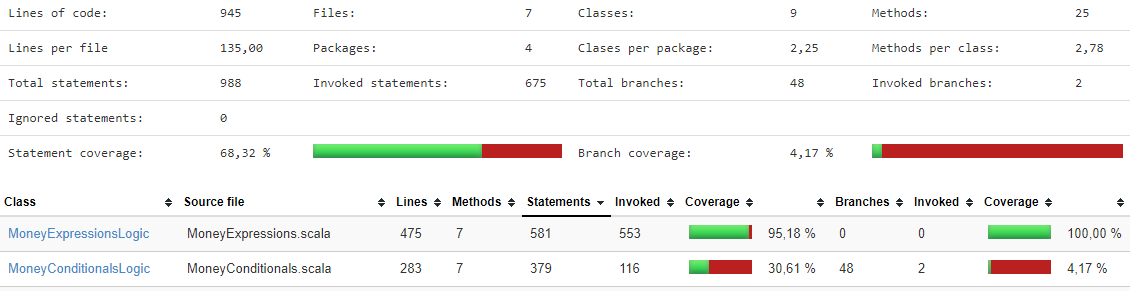
\includegraphics[width=\linewidth]{figures/eval_experiment1}
}
\caption{Test coverage report of the first experiment}
\label{fig:ch5_eval_experiment1}
\centering
\end{figure}
\\
\pinfo{Overall 68\%, cannot be 100, but can be improved}
The overall coverage over the generated system is 68\%, however, note that the generated system is based on the properties that we defined and that the libraries that are being used by the generated system are not included in the coverage report. The generated system also contains some other logic that is more related to how it communicates with other instances when it is deployed, which is not something that we test. As a result, we will not be able to bring the test coverage to 100\%. Although the test suite can be improved to have a higher test coverage, by generating values such that the properties using implication are also triggering the if-clause. Which is currently not the case, as we have seen when checking the coverage of each property in Figure X-1.\\
\\
\pinfo{\# of bugs, 4}
The second criteria that we defined was the amount of bugs that we have found by doing the experiment. By using this approach we found a total of 4 bugs. A compilation error, overflow/underflow error and precision errors. 2 of these 4 bugs were related to the precision problem when using doubles, but one originated from the library that is used for the Money type, while the other is because the \textit{Percentage} type is translated to a \textit{Double}. Which is why we define these as 2 separate bugs. An improvement of the test suite to also cover the properties using implication might result in more bugs that can be found. 


%\improvement{Comes out of the blue. Why this is done? Why exactly these changes? Tabular representation maybe?}
%Additional to the errors that we found in the generated system, we should be able to find bugs in the generator in case an expression is being incorrectly translated. We can easily test this by modifying the generator such that this is the case. So if we modify the translation of the "$\geq$" operator to "$>$", the result is 8 failing tests. But if we translate the "$\geq$" to "$\leq$" there will still be 7 failing tests. So to cover this, we would need more properties to test which focuses on the implementation of these operators.\change{What is done here? Change it. Not clear what the 8 tests and 7 tests mean. And why has this been done? Describe decisions}\\











